
%(BEGIN_QUESTION)
% Copyright 2006, Tony R. Kuphaldt, released under the Creative Commons Attribution License (v 1.0)
% This means you may do almost anything with this work of mine, so long as you give me proper credit

A common form of measurement error in instruments is called {\it hysteresis}.  A very similar type of measurement error is called {\it deadband}.  Describe what these errors are, and differentiate between the two.

\underbar{file i00091}
%(END_QUESTION)





%(BEGIN_ANSWER)

Hysteresis and dead band are not exactly the same type of calibration error, but they are closely related.  ``Dead band'' refers to a range of instrument measurement during reversal of input where the output does not change at all.  A common example of this is a ``loose'' steering system in an automobile, where the steering wheel must be turned excessively to take up ``backlash'' (mechanical slack) in the linkage system.  

Hysteresis refers to the situation where a reversal of input causes an immediate, but not proportionate, reversal of output.  This is commonly seen in air-actuated valves, where air pressure acts against the action of a large spring to precisely position a valve mechanism.  Ideally, the valve mechanism will move proportionally to the air pressure signal sent to it, and this positioning will be both repeatable and accurate.  Unfortunately, friction in the valve mechanism produces hysteresis: a different air pressure signal may be required to position the valve mechanism at the same location opening versus closing, but unlike dead band, {\it any} amount of signal reversal (change of direction: increasing vs. decreasing) will cause the valve to move slightly.

Compare the following transfer function graphs to understand the difference between hysteresis and dead band:

$$\includegraphics[width=15.5cm]{i00091x01.eps}$$

Both dead band and hysteresis are characteristically mechanical phenomena.  Electronic circuits rarely exhibit such ``artifacts'' of measurement or control.  Dead band and hysteresis are more often found together than separately in any instrument.

Interestingly, both effects are present in magnetic circuits.  The magnetization curves for typical transformer core steels and irons are classic examples of hysteresis, whereas the magnetization curve for ferrite (in the saturation region) is quite close to being a true representation of deadband.

%(END_ANSWER)





%(BEGIN_NOTES)


%INDEX% Calibration, deadband: definition
%INDEX% Calibration, hysteresis: definition

%(END_NOTES)


